
\section{Tasks}
\label{cp6:tasks}



We opted for an experiment with tasks that could be completed by participants on their own time and computer.
This decision was motived by the COVID-19 pandemic and the need for social distance\red{~\cite{}}. 
Hence, we decided to use tasks that are easy to understand and perform in a single experimental session, but that still required a participant  
to seek information in artifacts associated with that task.

% 


Based on these criteria and guided by~\cite{thiselton2019},
Table~\ref{tbl:python-tasks-modules} details the tasks that we have selected. 
These tasks are based on 
Python w3resource\footnote{\url{https://www.w3resource.com/python-exercises/}} tasks
that require usage of at least one module external to the Python core library.
By using external modules, we aim to reduce the likelihood that a participant 
can provide a solution for a task without consulting any of the artifacts
that detail how to use such modules (Section~\ref{cp6:experiment-artifacts}). 







% We chose these tasks due to how they focus on modules widely adopted both by open source systems and by private companies.
% As an example, the \texttt{NYTimes} task involves using a HTML parser, namely \texttt{BeautifulSoup},
% which Reddit---a social news aggregator with approximately 430 million monthly users---uses 
% to parse urls and identify images shown on its posts' headlines~\cite{bs4-reddit}. 




While we leave details about the procedures associated with manual and tool-assisted tasks to another section, Figure~\ref{fig:nytimes-task-colab} provides an excerpt of the information shown in a task\footnote{Full descriptions are available in the experiment's supplementary material~\red{\cite{}}.}.
For each task, participants had the task description and examples of input and output scenarios at their disposal. A task contained a list of resources (Section~\ref{cp6:experiment-artifacts}) that participants could consult 
so that they could come up with a solution for the task.
Each task also contained a link to an online coding environment
where they could write and test their solution (Section~\ref{cp6:coding-environment}). 




\begin{table}
\centering
\caption{Python tasks}
\begin{footnotesize}
\rowcolors{2}{}{lightgray}
\begin{tabular}{ll}
\hline
\textbf{Task} & \textbf{Description}                                                                                         \\
\hline
\hline
%
\parbox[l][1cm][c]{1cm}{Practice task}       &
\parbox[l][1cm][c]{11cm}{Given three dictionaries representing address books,
you must write an algorithm using the Python core \texttt{dict} module to merge them.}    \\
\hline
%
Distances     &
\parbox[l][1.3cm][c]{11cm}{Given a string representing a rendezvou point and a list of suggested picnic addresses
    you must write an algorithm using the \texttt{geopy} module to find the  picnic address closest to the rendezvou point.} \\
%
NYTimes       &
\parbox[l][1cm][c]{11cm}{Given a string representing the url for NY Times Today's,
    write an algorithm using the \texttt{BeautifulSoup} and \texttt{requests} modules to scrape all the headlines of that page.}
\\
%
Titanic       &
\parbox[l][1cm][c]{11cm}{Given a string representing a url for the titanic dataset,
    you must write an algorithm using the \texttt{pandas} and \texttt{seaborn} modules to create a barchart of the data.}    \\
    
\hline
\end{tabular}
\end{footnotesize}
% \smallskip
\label{tbl:python-tasks-modules}
\end{table}









\subsection{Artifacts}
\label{cp6:experiment-artifacts}


Each task requires a set of artifacts that a participant could peruse for information that could assist them complete the task.
We select artifacts for a task following procedures similar to the ones we used to create the \acs{DS-android} dataset (Chapter~\ref{ch:android-corpus}). 
For each of the tasks in Table~\ref{tbl:python-tasks-modules}, we use the Google search engine to obtain up to ten artifacts that likely contain relevant
information for that task. 







\subsection{Coding environment}
\label{cp6:coding-environment}






To ensure that participants had the same conditions to perform each task
and also to minimize setup instructions, we used Google Colab\footnote{\url{https://colab.research.google.com/}} as our coding environment. 



% Figure~\ref{fig:nytimes-task-colab} shows an example of our online environment.
% At the left-hand side, 
% where they had a code editor with amenities commonly found in modern IDEs, such as code completion and syntax highlighting. 



Colab provided participants with a code editor with amenities commonly found in modern IDEs, e.g., code completion and syntax highlighting. It also ensured that all the participants 
performed the tasks in the same Python version and it lifted 
burdens that could arise from installing dependencies associated with the external modules used in each of our tasks. 



Figure~\ref{fig:nytimes-task-colab} shows an example of the Colab coding environment. 
First it handled dependencies management and then, 
it presented a class containing a single method with a \texttt{TODO} block where 
participants should write their solution. 
The environment also provided a main function where participants could see the output
of their code. Alternatively, a participant could use test cases to test their solution
against the examples shown alongside the task description.
% Upon testing, the system would display full details about the test cases, e.g., the test's input, which assertion failed, and why. 





\clearpage

\begin{figure}
    \centering
    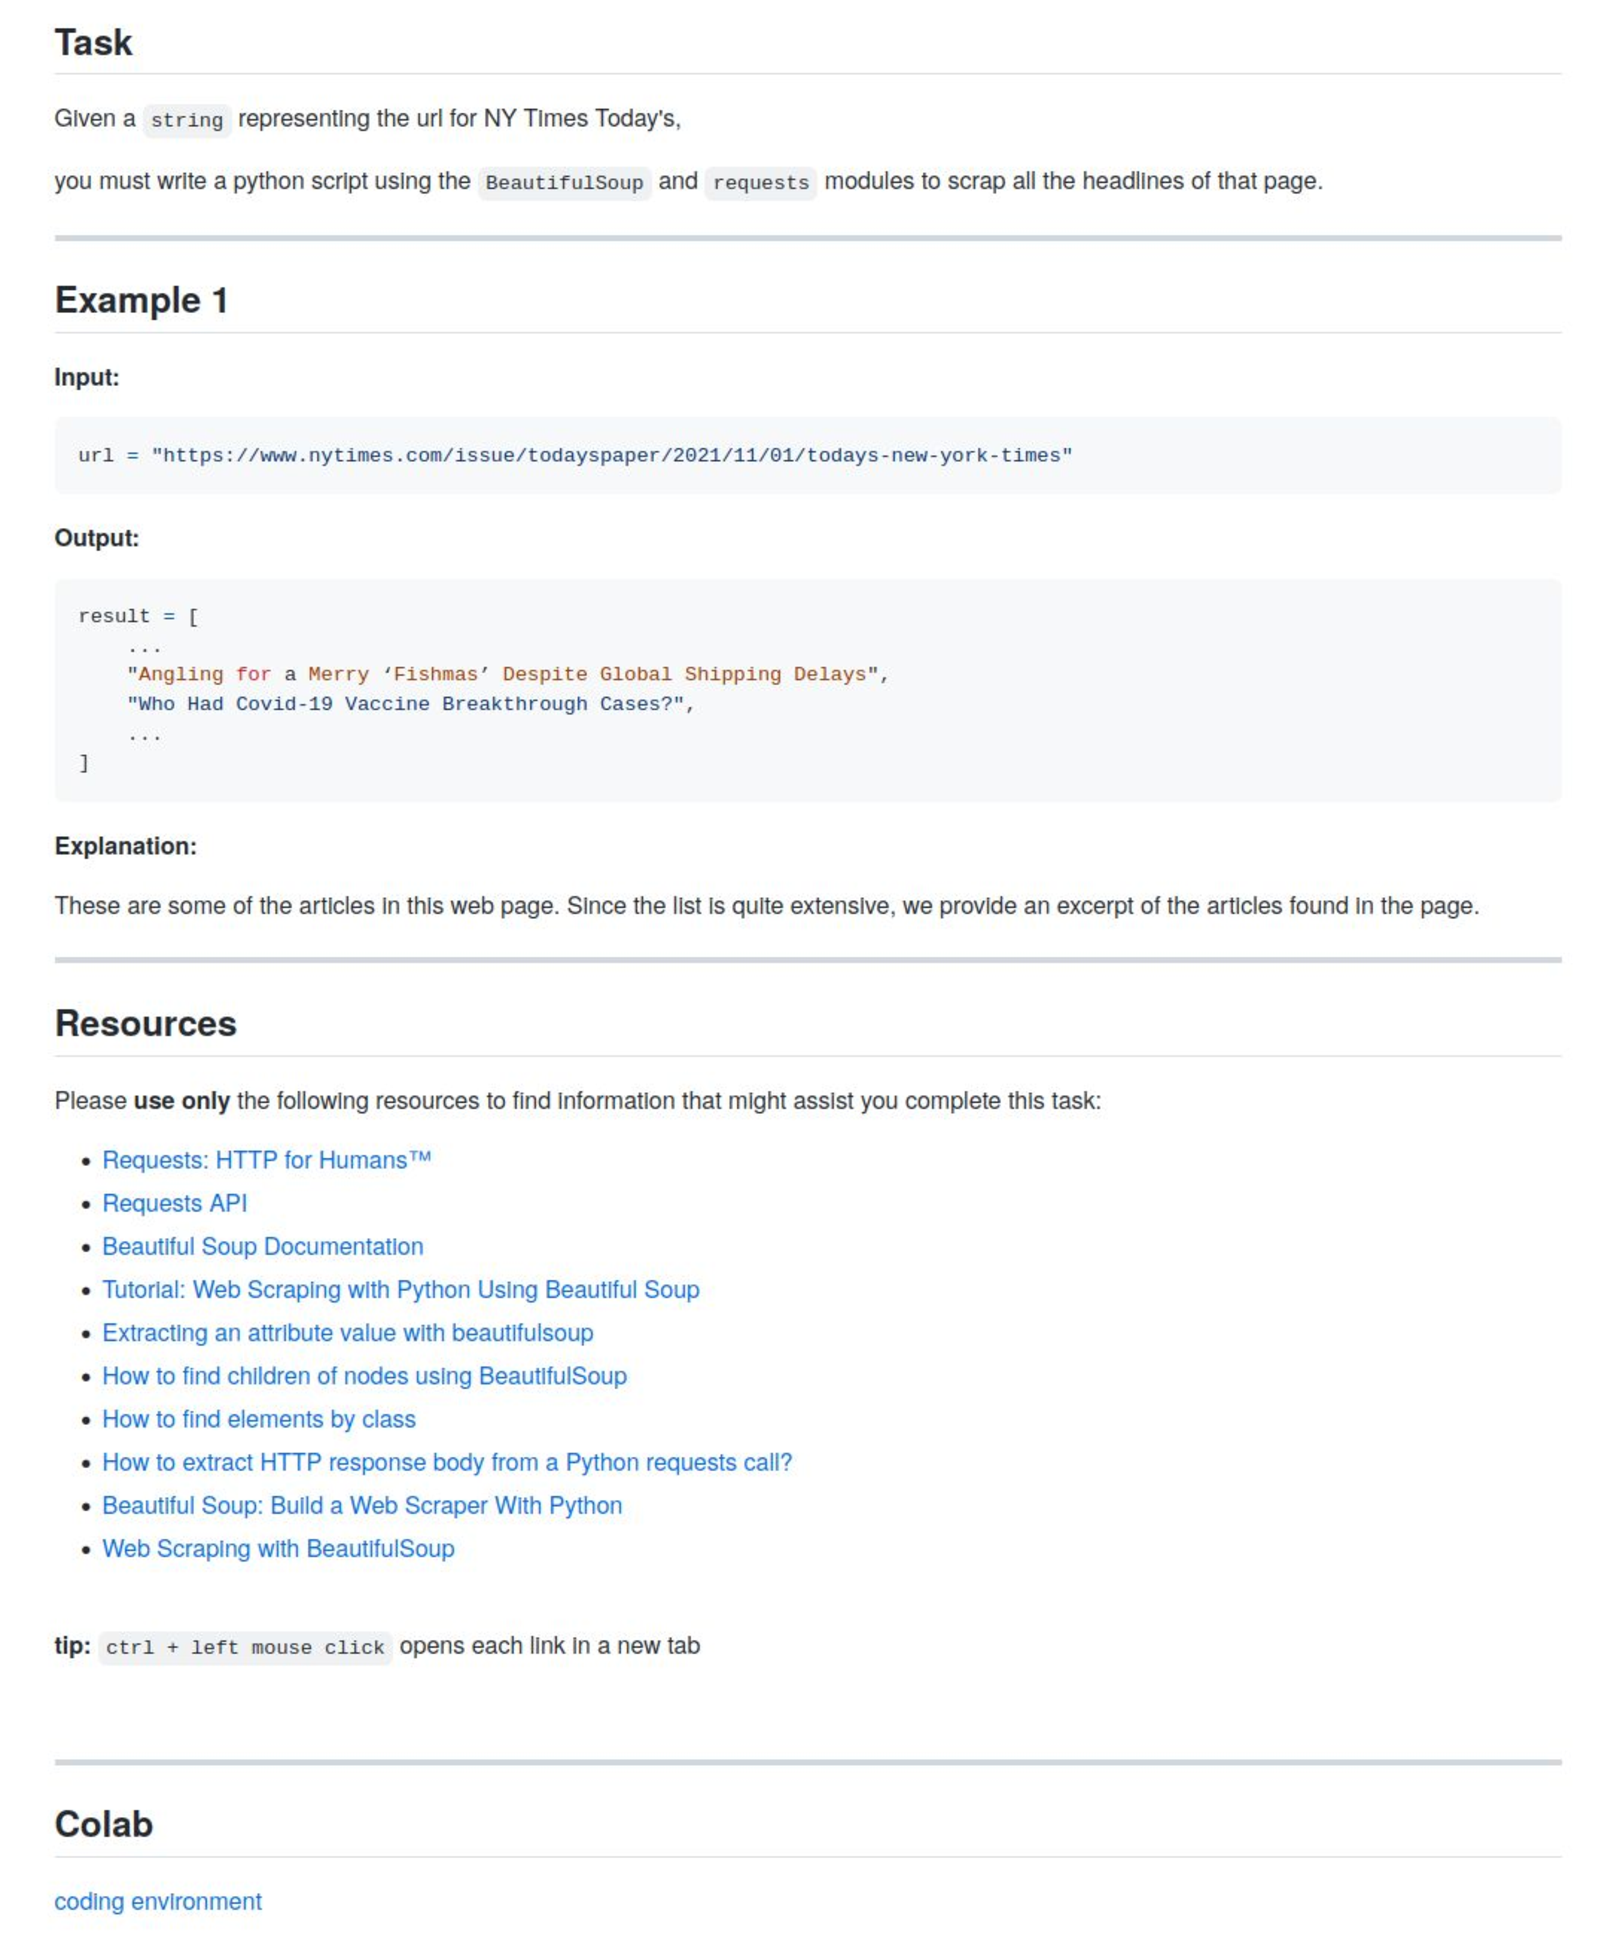
\includegraphics[width=1\textwidth]{cp6/task-github.pdf}
    \caption{Information shown in a task}
    \label{fig:nytimes-task-colab}
\end{figure}



\clearpage

\begin{figure}
    \centering
    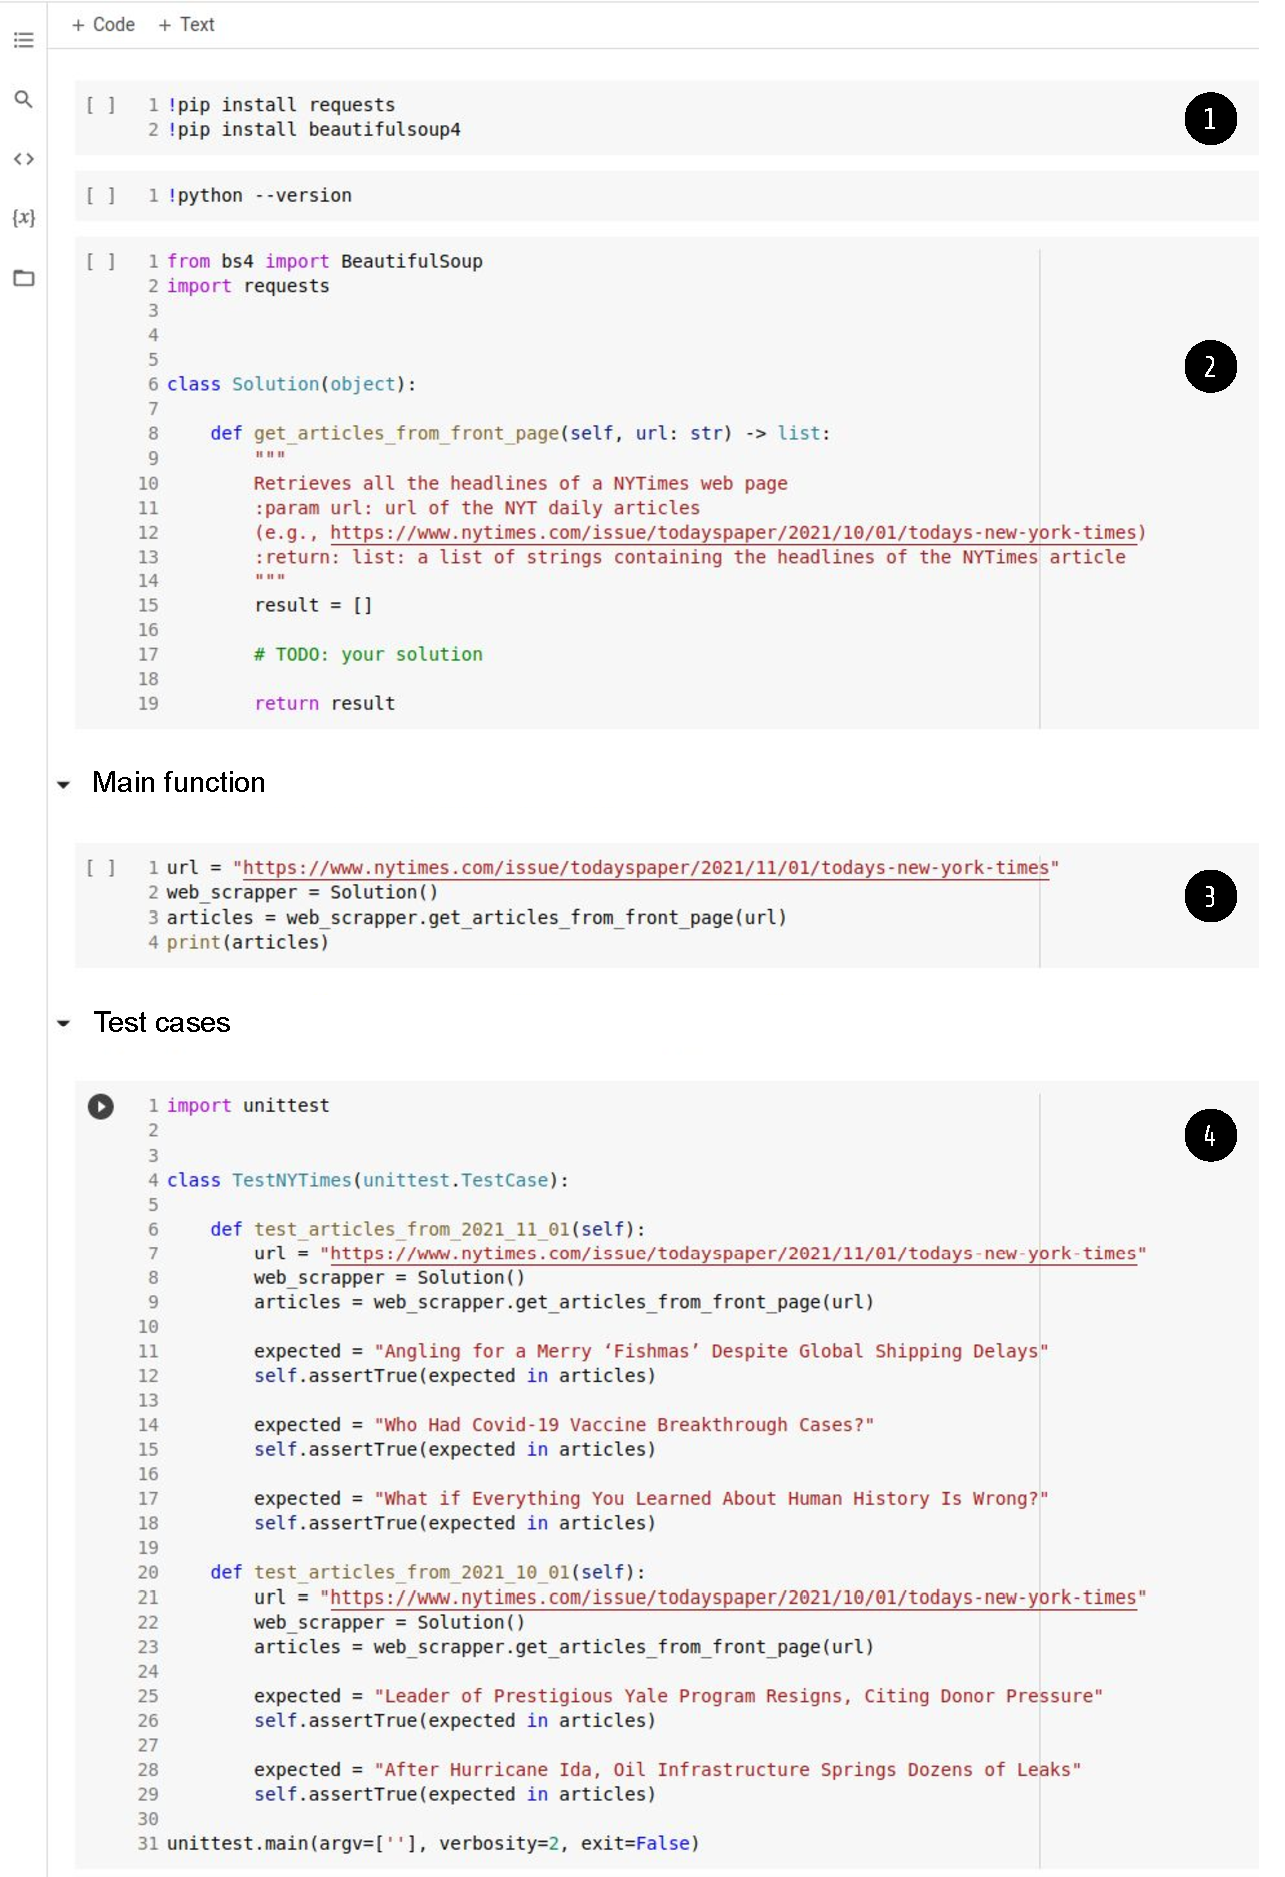
\includegraphics[width=\textwidth]{cp6/task-colab.pdf}
    \caption{Colab environment}
    \label{fig:nytimes-task-colab}
\end{figure}



\clearpage



% Similarly, the \texttt{Titanic} task encompasses using \texttt{Pandas}, a data analysis and manipulation module
% used in many open source data science projects~\cite{ma2017, shrestha2020}.